% tGISguide.tex
% v3.4 released April 2009

\documentclass[]{tGIS2e}


\citestyle{tGIS}
\begin{document}

\doi{10.1080/1365881YYxxxxxxxx}
\issn{1362-3087} \issnp{1365-8816} \jvol{00} \jnum{00} \jyear{2009} %\jmonth{February}

\markboth{Taylor \& Francis and I.T. Consultant}{International Journal of Geographical Information Science}

\articletype{GUIDE}

\title{{\itshape International Journal of Geographical Information Science} -- \LaTeXe\ style guide
for authors\newline (Style 2 + References Style V)}

\author{Taylor \& Francis$^{a}$$^{\ast}$\thanks{$^\ast$Corresponding author. Email: latex.helpdesk@tandf.co.uk
\vspace{6pt}} and I.T. Consultant$^{b}$\\\vspace{6pt}  $^{a}${\em{4 Park Square, Milton Park, Abingdon, UK}};
$^{b}${\em{Institut f\"{u}r Informatik, Albert-Ludwigs-Universit\"{a}t, Freiburg,
Germany}}\\\vspace{6pt}\received{v2.3 released April 2009} }

\maketitle

\begin{abstract}
This guide 
\end{abstract}

\noindent{\bf{Please note that the index following the abstract in this guide is provided for information only. An index is not required in submitted papers.}}

\section{Introduction}

All submissions of manuscripts for possible publication in {\itshape International Journal of Geographical Information Science} ({\it tGIS}\,)  should be made online via the journal's Manuscript Central site ({\tt{http://mc.manuscriptcentral.com/ijgis}}). New users should first create an account. Once logged on to the site, submissions should be made via the Author Centre. Online user guides and access to a helpdesk are available on this website.

{\it tGIS} accepts papers in any standard format, including Microsoft$\circledR$ Word, PostScript and PDF. Files submitted in formats other than PDF will automatically be converted to a PDF for the review process. \LaTeXe\ files should be converted to PDF prior to submission because Manuscript Central is not able to convert \LaTeXe\ files into PDFs directly. This journal does not accept Microsoft Word 2007 documents. Please use Word's `Save As' option to save your document as an older (.doc) file type. For the submission of manuscripts created using \LaTeXe\, see Section~\ref{S1.2}.

The layout design for {\it tGIS} has been implemented as a \LaTeXe\ Class file. The {\it tGIS} Class file is
based on {\tt article.cls}. Commands that differ from the standard \LaTeXe\ interface, or which are provided in
addition to the standard interface, are explained in this guide. This guide is not a substitute for the \LaTeXe\
manual itself.

This guide can be used as a template for composing an article for submission by cutting, pasting, inserting and
deleting text as appropriate, using the LaTeX environments provided (e.g. \verb"\begin{equation}",
\verb"\begin{corollary}").\vspace{6pt}

\subsection{The {\bi tGIS} document style}

The use of \LaTeXe\ document styles allows a simple change of style (or style option) to transform the appearance
of your document. The tGIS2e Class file preserves the standard \LaTeXe\ interface such that any document that can
be produced using the standard \LaTeXe\ {\tt article} style can also be produced with the {\it tGIS} style.
However, the measure (or width of text) is narrower than the default for {\tt article}, therefore line breaks
will change and long equations may need re-formatting.

When your article appears in the print edition of the {\it gPAV} journal (and exactly reproduced in the PDF
version online), it will have been typeset in Monotype Times. As most authors do not own this font, it is inevitable that the page make-up will change with the change of font. For this reason, we ask authors to ignore details such as slightly long lines, page stretching, or figures falling out of synchronization with their citations in the text, because these details will be dealt with during proofing.

\subsection{Submission of \LaTeXe\ articles to the journal}\label{S1.2}

All submissions of manuscripts for possible publication should be made online via the journal's Manuscript Central site ({\tt{http://mc.manuscriptcentral.com/ijgis}}). New users should first create an account. Once logged on to the site, submissions should be made via the Author Centre. Online user guides and access to a helpdesk are available on this website. \LaTeXe\ files should be converted to PDF prior to submission because Manuscript Central is not able to convert \LaTeXe\ files into PDFs directly. The PDF should be uploaded together with the \LaTeXe\ source files and any graphics files.

General Instructions for Authors may be found at
\begin{center}(\nobreak{\tt{http://www.tandf.co.uk/journals/authors/tgisauth.asp}}).\end{center}

Only `open-source' \LaTeXe\ should be used, not proprietary systems such as TCI LaTeX or Scientific WorkPlace. Similarly, Class files such as REVTex4 that produce a document in the style of a different publisher and journal should not be used for preference.

Appropriate gaps should be left for figures, of which original versions and copies should also be supplied.
Authors should ensure that their figures are suitable (in terms of lettering size, etc.) for the reductions they
intend.

Authors who wish to incorporate Encapsulated PostScript artwork directly in their articles can do so by using
Tomas Rokicki's {\tt EPSF} macros (which are supplied with the DVIPS PostScript driver). See Section~\ref{eps},
which also demonstrates how to treat landscape pages. Please remember to supply any additional figure macros you
use with your article in the preamble before \verb"begin{document}". Authors should not attempt to use
implementation-specific \verb"\special"'s directly.

Ensure that any author-defined macros are gathered together in the source file, just before the
\verb"\begin{document}" command.

Please note that, if serious problems are encountered with the coding of a paper (missing author-defined macros,
for example), it may prove necessary to divert the paper to conventional typesetting, i.e. it will be re-keyed.

\section{Using the {\bi tGIS} Class file}

If the file {\tt tGIS2e.cls} is not already in the appropriate system directory for \LaTeXe\ files, either
arrange for it to be put there, or copy it to your working folder. The {\it tGIS} document style is implemented
as a complete document style, {\em not\/} a document style option. In order to use the {\it tGIS} style, replace
{\tt `article'} by {\tt `tGIS2e'} in the \verb"\documentclass" command at the beginning of your document:
%
\begin{verbatim}
\documentclass{article}
\end{verbatim}
%
is replaced by
%
\begin{verbatim}
\documentclass{tGIS2e}
\end{verbatim}
%
In general, the following standard document style options should {\em not\/} be used with the {\it tGIS} style:
%
\begin{enumerate}
   \item {\tt 10pt}, {\tt 11pt}, {\tt 12pt} -- unavailable;
   \item oneside (no associated style file) -- oneside is the default;
   \item {\tt leqno} and {\tt titlepage} -- should not be used;
   \item {\tt singlecolumn} -- is not necessary as it is the default style.
\end{enumerate}
%

\subsection{Landscape pages}\label{eps}

If a table or illustration is too wide to fit the standard measure, it must be turned, with its caption, through
90$^{\circ}$ anticlockwise. Landscape illustrations and/or tables can be produced directly using the tGIS2e style
file using \verb"\usepackage{rotating}" after \verb"\documentclass{tGIS2e}". The following commands can be used
to produce such pages.
%
\begin{verbatim}
\setcounter{figure}{2}
\begin{sidewaysfigure}
\centerline{\epsfbox{fig1.eps}}
\caption{This is an example of figure caption.}
\label{landfig}
\end{sidewaysfigure}
\end{verbatim}
%
\begin{verbatim}
\setcounter{table}{0}
\begin{sidewaystable}
  \tbl{The Largest Optical Telescopes.}
    \begin{tabular}{@{}llllcll}
    .
    .
    .
  \end{tabular}\label{tab1}
\end{sidewaystable}
\end{verbatim}
%
Before any float environment, use the \verb"\setcounter" command
as above to fix the numbering of the caption. Subsequent captions
will then be automatically renumbered accordingly.


\section{Additional features}

In addition to all the standard \LaTeXe\ design elements, {\it tGIS} style includes a separate command for specifying short versions of the authors' names and the journal title for running headlines on the left-hand (verso) and right-hand (recto) pages, respectively (see Section~\ref{markboth}).  In general, once you have used this additional {\tt tGIS2e.cls} feature in your document, do not process it with a standard \LaTeXe\ style file.

\subsection{Footnotes to article titles and authors' names}

On the title page, the \verb"\thanks" control sequence may be used to produce a footnote to either the title or authors' names.

\vspace{6pt}Footnote symbols should be used in the order: $\dagger$
(coded as \verb"\dagger"),\break $\ddagger$ (\verb"\ddagger"), $\S$ (\verb"\S"),
$\P$ (\verb"\P"), $\|$ (\verb"\|"), $\dagger\dagger$
(\verb"\dagger\dagger"),\break $\ddagger\ddagger$
(\verb"\ddagger\ddagger"),  $\S\S$ (\verb"\S\S"), $\P\P$ (\verb"\P\P"),
$\|\|$ (\verb"\|\|").

Note that footnotes to the text will automatically be assigned the superscript
 symbols 1, 2, 3,... by the Class file, beginning afresh on each
page.\footnote{These symbols will be changed to the style of the journal by the
 typesetter during preparation of your proofs.}

The title, author(s) and affiliation(s) should be followed by the {\verb"\maketitle"} command.

\subsection{Abstracts}

At the beginning of your article, the title should be generated in the usual way using the {\verb"\maketitle"}
command. Immediately following the title you should include an abstract. The abstract should be enclosed within
an {\tt abstract} environment. For example, the titles for this guide were produced by the following source code:
%
\begin{verbatim}

\title{{\itshape International Journal of Geographical Information %
Science} -- \LaTeXe\ style guide for authors\newline (Style 2 + %
References Style V)}

\author{Taylor \& Francis$^{a}$$^{\ast}$\thanks{$^\ast$Corresponding %
author. Email: latex.helpdesk@tandf.co.uk \vspace{6pt}} and I.T. %
Consultant$^{b}$\\\vspace{6pt}  $^{a}${\em{4 Park Square, Milton Park, %
Abingdon, UK}}; $^{b}${\em{Institut f\"{u}r Informatik, %
Albert-Ludwigs-Universit\"{a}t, Freiburg, Germany}}\\\vspace{6pt}%
\received{v2.3 released April 2009} }



\maketitle
\begin{abstract}
This guide is for authors who are preparing papers for the Taylor \& %
Francis journal {\em International Journal of Geographical Information %
Science} ({\it tGIS}\,) using the \LaTeXe\ document preparation system %
and the Class file {\tt tGIS2e.cls}, which is available via the journal %
homepage on the Taylor \& Francis website (see Section~\ref{FTP}). %
Authors planning to submit their papers in \LaTeXe\ are advised to %
use {\tt tGIS2e.cls} as early as possible in the creation of their %
files. \end{abstract}

\end{verbatim}

\noindent{\bf{(Please note that the percentage signs at the ends of lines that quote source code in this document are not part of the coding but have been inserted to achieve line wrapping at the appropriate points.)}}

\subsection{Lists}

The {\it tGIS} style provides numbered and unnumbered lists using the {\tt enumerate} environment and bulleted
lists  using the {\tt itemize} environment.

The enumerated list numbers each list item with arabic numerals:
%
\begin{enumerate}
   \item first item
   \item second item
   \item third item
\end{enumerate}
%
Alternative numbering can be achieved by an argument in square brackets, e.g. \verb"\item[(i)] first item".
%
Unnumbered lists are also provided using the {\tt enumerate} environment.
For example,
\begin{enumerate}
   \item[] First unnumbered indented item without label.
   \item[] Second unnumbered item.
   \item[] Third unnumbered item.
\end{enumerate}
was produced by:
%
\begin{verbatim}
\begin{enumerate}
  \item[] First unnumbered indented item...
  \item[] Second unnumbered item.
  \item[] Third unnumbered item.
\end{enumerate}
\end{verbatim}
%
Bulleted lists are provided using the {\tt itemize} environment. For example,
\begin{itemize}
\item First bulleted item
\item Second bulleted item
\item Third bulleted item
\end{itemize}
was produced by:
\begin{verbatim}
  \begin{itemize}
  \item First bulleted item
  \item Second bulleted item
  \item Third bulleted item
  \end{itemize}
\end{verbatim}


\section[]{Some guidelines for using standard features}

The following notes may help you achieve the best effects with the tGIS2e Class file.





%\begin{figure}
%\begin{center}
%\vspace{36pt}
%\begin{minipage}{100mm}
%\subfigure[]{
%\resizebox*{5cm}{!}{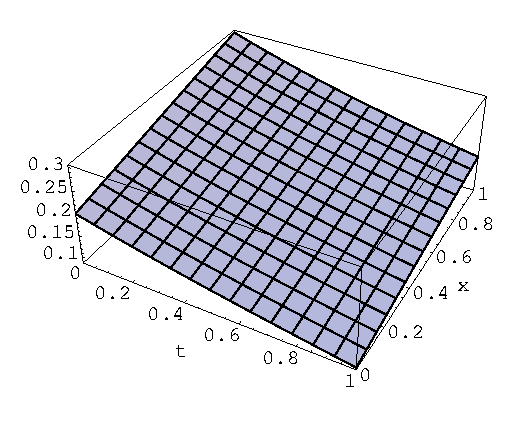
\includegraphics{senu_gr1.eps}}}%
%\subfigure[]{
%\resizebox*{5cm}{!}{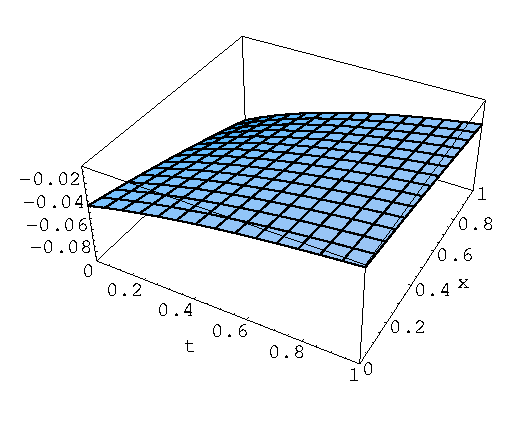
\includegraphics{senu_gr2.eps}}}%
%\caption{Example of a two-part figure with individual %
%sub-captions showing that all lines of figure captions range left.}%
%\label{sample-figure}
%\end{minipage}
%\end{center}
%\end{figure}





\subsection{Acknowledgements}
zz




\subsection{References}\label{refs}
\begin{thebibliography}{9}

\markboth{Taylor \& Francis and I.T. Consultant}{International Journal of Geographical Information Science}

\bibitem[\protect\citeauthoryear{Agutter}{1995}]{Agu95}
Agutter, A.J., 1995. The linguistic significance of current British slang.
  Thesis (PhD). Edinburgh University, UK.

\bibitem[\protect\citeauthoryear{Cutler {\itshape{et~al.}}}{1986}]{cww86}
Cutler, T., Williams, K., and Williams, J., 1986. {\itshape Keynes, Beveridge and
  beyond}. 3rd ed. Twentieth century political economics Vol. II. London:
  Routledge.

\bibitem[\protect\citeauthoryear{Evans}{1994}]{ev94}
Evans, W.A., 1994. Approaches to intelligent information retrieval. {\itshape
  Information Processing and Management}, 7 (2), 147--168.

\bibitem[\protect\citeauthoryear{French}{1988}]{fzf88}
French, F., 1988. English title of a chapter in the translation of a book in a
  foreign language.  {\itshape{In}}: {\itshape Title of a book in another language (Quoted in
  that language)}  [{\itshape English translation}],  translated by P. Smith.
  New York: Dover (original work published 1923).

\bibitem[\protect\citeauthoryear{Glover and Ribeiro}{1951}]{GloRib51}
Glover, F. and Ribeiro, C.C., eds, 1951. {\itshape
Lessons of the British war economy}. 2nd ed. Westport, CT: Greenwood Press, 1--24.

\bibitem[\protect\citeauthoryear{Holland}{2004}]{Holl04}
Holland, M., 2004. {\itshape Guide to citing Internet sources} [online]. Poole, UK: Bournmouth University. Available from:
  http://www.bournemouth.ac.uk/library/using/guide\_to\_citing\_internet\_sourc.%
  html [Accessed 4 November 2004].

\bibitem[\protect\citeauthoryear{Kern}{1997}]{hk97}
Kern, H., 1997. The resurgent Japanese economy and a Japan--United States free trade
  agreement. {\itshape {In}}: C.~Lambert and G.~Holst, eds. {\itshape 4th international conference on the restructuring of the economic and political system in Japan}, Milan, Italy, 21--25 May 1996. Singapore: World Scientific, 147--156.

\bibitem[\protect\citeauthoryear{Korb}{1995}]{Kor95}
Korb, K.B., 1995. Persons and things: book review of Bringsjord on
  robot-consciousness. {\itshape Psycoloquy} [online], 6 (15). Available from: http://psycprints.ecs.soton.ac.uk/archive/00000462/ [Accessed 20 May 2004].

\bibitem[\protect\citeauthoryear{Misner}{1973}]{cwm73}
Misner, C.W., ed., 1973. Efficient algorithms for layer assignment problems. {\itshape{In}}:
  {\itshape Gravitation in a collapsing Universe}. San Francisco, CA:
  Freeman.

\bibitem[\protect\citeauthoryear{Patel}{2002}]{fwp02}
Patel, F.W., 2002. {\itshape Banking technology in an age of cynicism}. Mongraphs on
  technical aspects Vol. XIII. New York: Dover.

\bibitem[\protect\citeauthoryear{Pierce {\itshape{et~al.}}}{1976}]{PeaEtAl76}
Pierce, I.F., {\itshape{et al.}}, 1976. A
  model of output, employment, wages and prices in the UK. {\itshape{In}}: M.~Laguna and
  J.L. Gonz\'{a}les-Velarde, eds. {\itshape Computing tools for modeling, optimization and simulation: interfaces in
  computer science and operations research}. 2nd  ed. Boston, MA: Cambridge University
  Press, 1--24.
\end{thebibliography}

%\markboth{Taylor \& Francis and I.T. Consultant}{International Journal of Geographical Information Science}




\label{lastpage}

\end{document}
